\documentclass[runningheads,a4paper]{llncs}

\usepackage{amssymb}
\setcounter{tocdepth}{3}
\usepackage{graphicx}

\usepackage{url}
\urldef{\mailsa}\path|{amherag, mario}@tectijuana.edu.mx,alejandra.mancilla@gmail.com|
%\urldef{\mailsa}\path||
%\urldef{\mailsa}\path|{alfred.hofmann, ursula.barth, ingrid.haas, frank.holzwarth,|
%\urldef{\mailsb}\path|anna.kramer, leonie.kunz, christine.reiss, nicole.sator,|
%\urldef{\mailsc}\path|erika.siebert-cole, peter.strasser, lncs}@springer.com|    
\newcommand{\keywords}[1]{\par\addvspace\baselineskip
\noindent\keywordname\enspace\ignorespaces#1}

\begin{document}

\mainmatter  % start of an individual contribution

% first the title is needed
\title{Affective States in Software Programming: Classification of Individuals based on their Keystroke and Mouse
Dynamics}

% a short form should be given in case it is too long for the running head
\titlerunning{Affective States in Software Programming: Classification of Individuals based on their Keystroke and Mouse
Dynamics}

% the name(s) of the author(s) follow(s) next
%
% NB: Chinese authors should write their first names(s) in front of
% their surnames. This ensures that the names appear correctly in
% the running heads and the author index.
%
\author{Amaury Hernandez-Aguila%
%\author{}%
\and Mario Garcia-Valdez\and Alejandra Mancilla}
%
\authorrunning{Affective States in Software Programming: Classification of Individuals based on their Keystroke and Mouse
Dynamics}
% (feature abused for this document to repeat the title also on left hand pages)

% the affiliations are given next; don't give your e-mail address
% unless you accept that it will be published
\institute{Instituto Tecnológico de Tijuana\\
Calzada Tecnologico s/n, Tijuana, Mexico\\
%\institute{
\mailsa\\
\mailsb\\
\mailsc\\
\url{}}

%
% NB: a more complex sample for affiliations and the mapping to the
% corresponding authors can be found in the file "llncs.dem"
% (search for the string "\mainmatter" where a contribution starts).
% "llncs.dem" accompanies the document class "llncs.cls".
%

\toctitle{Lecture Notes in Computer Science}
\tocauthor{Authors' Instructions}
\maketitle


\begin{abstract}
  In this paper, a method is presented for the classification of an individual into two affective states: boredom and frustration. To gather the necessary data, the individual interacts with an Intelligent Tutoring System focused on the teaching of programming languages. The method involves a classifier based on k-NN, and feature vectors generated by the preprocessing of keystroke dynamics and mouse dynamics data. Accurate results are achieved by determining relevant subsets of the initial feature set, using genetic algorithms. These subsets facilitate the training of the classifiers for each affective state.
\keywords{Affective Computing, Intelligent Learning Environments, Keystroke Dynamics, Mouse Dynamics, k-Nearest Neighbors}
\end{abstract}


\section{Introduction}
 
The recognition and simulation of human affects are becoming important fields of study, as many researchers have demonstrated that affect-aware computers can provide better performance in assisting humans \cite{affective-computing}. There are works describing different approaches for the recognition and simulation of affective states in human beings. For example El Kaliouby and Robinson \cite{facial-expressions} proposed a system based on Dynamic Bayesian Networks (DBN) that successfully recognized affective states from a video stream of facial expressions and head gestures in real-time. A work aimed at the simulation of affective states is by Becker-Asano and Wachsmuth \cite{affective-simulation} who created MAX, a virtual human that simulates emotions in congruence to the mood of the person that interacts with it.
%Falta añadir una explicación de affective recognition (primera nota)

It didn't take long before these techniques were implemented as components of Intelligent Learning Environments (ILE), as the recognized affective states can be used as part of the students' user model. D'Mello, et al. \cite{autotutor} present the development of an affect-sensitive Intelligent Tutoring System (ITS) called AutoTutor, which recognizes the emotions of a learner by monitoring conversational cues, gross body language, and facial features, and attempts to address the presence of negative emotional states with empathetic and motivational statements. Additionally, Drummond and Litman \cite{zoning-out} explain a method based on machine learning classification models to asses if a student is zoning out during a spoken learning task.

But as more ILEs embrace these methodologies and techniques pertaining to the field of study known as Affective Computing \cite{affective-computing}, a problem arises. In order to perform a recognition of the users' affective states, a sensor must be used to gather data. Frequently, these sensors can be considered as intrusive or invasive \cite{intrusive1} \cite{intrusive2} \cite{intrusive3}, and can disrupt the learning experience of a student. In this work, a method is proposed for the recognition of affective states based on Keystroke and Mouse Dynamics. Keyboard and mouse input devices should address the problem of the intrusive nature of most sensors, as the vast majority of an ILE's users should be familiarized with the use of this hardware equipment nowadays, and should not regard them as an abnormal factor in the learning environment.

Research works related to Keystroke Dynamics (KD) are carried out either using fixed-texts, or free-texts \cite{free-text-fixed-text}. KD performed on fixed-texts involves the recognition of typing patterns when typing a pre-established fixed-length text, e.g., a password. In the other case, free-text KD achieves the recognition of typing patterns when typing an arbitrary-length text, e.g., a description of an item. However, as noted by Janakiraman and Sim \cite{fixed-is-better}, most of the research regarding KD is done on fixed-text input, the reason being that fixed-text KD usually yields better results than free-text KD. Yet, the authors of this work share the opinion with Janakiraman, R., and Sim, T., that it would be more useful if KD can handle free text as well as fixed text.

As a proof of concept for free-text KD, the method for the recognition of affective states presented in this work is performed in an ITS focused on the teaching of software programming, where students need to input arbitrary-length source code. In this ITS, a student is required to solve a series of programming exercises, and, according to a feature vector extracted from the processed Keystroke and Mouse Dynamics data, a classification of two affective states (boredom and frustration) of the student is accomplished. This classification involves determining if a student was experiencing or not each of the two affective states during the resolution of the programming exercises. With the proposed method, ILEs can predict a learner's affective states, and create better user models in order to provide adaptive, affect-sensitive content.

The structure of this work is organized as follows: Section \ref{related-work} presents a series of works related to the proposed method in this paper; Section \ref{proposed-method} describes the proposed method for the recognition of two affective states in an ITS for the teaching of programming languages; Section \ref{experiment} explains how an experiment was performed to demonstrate the proposed method, and Section \ref{results} presents the results; finally, a conclusion to this work can be found in Section \ref{conclusion}.

%Falta añadir esto

%Falta añadir el abstract

\section{Related Work}
\label{related-work}

Bosch, D'Mello and Mills \cite{emotions-novices-programming} analyzed the relationship between affective states and performance of novice programmers when they were learning the basics of computer programming in the Python language. The results of their study indicated that the more common emotions students experienced were engaged, confusion, frustration, and boredom, with 23\%, 22\%, 14\%, and 12\% of the students experiencing these emotions, respectively. It was useful to consider these results, as it gives evidence of what affective states to be targeted in order to obtain less biased data. For example, if a less common emotion was chosen, a classifier could opt to classify any feature vector as not experiencing such emotion. Nevertheless, the classifier would obtain accurate results, although the classifier would be inaccurate at determining if a feature vector was actually experiencing the given affective state.

Similar to the previous work, Rodrigo, et al. \cite{emotions-novices-programming2} observed which affective states and behaviors relate to student's achievement within a Computer Science course. The authors found that confusion, boredom and engagement in IDE-related on-task conversation are associated with lower achievement.

Although the use of Keystroke Dynamics (KD) can be found in several research works as a biometric measure, its use as a mechanism for identifying affective states is rare in comparison. Epp, Lippold and Mandryk \cite{keystroke-dynamics1} effectively used KD in conjunction with decision-tree classifiers for the identification of 15 affective states. Although their work was based on fixed-text KD, their decisions on how to extract a feature set from the data generated by the KD process was an inspiration for the proposed method in this work. As for free-text KD, Bixler and D'Mello \cite{keystroke-dynamics2} present a method for the identification of boredom and engagement based on several classification models.

Regarding Mouse Dynamics (MD), some research has been conducted for the identification of affective states, although, as with the case of KD, MD is mainly used as a biometric measure for authentication processes. Salmeron-Majadas, Santos and Boticario \cite{mouse-dynamics1} use both MD and KD to predict four affective states using five different classification algorithms. Bakhtiyari and Husain \cite{mouse-dynamics2} discuss a method based on fuzzy models for the recognition of emotions through KD, MD and touch-screen interactions. For a broad review of emotion recognition methods based on KD and MD, the work by Kolakowska \cite{keystroke-mouse-review} is recommended.

%% It has to be mentioned that a numerous list of works pertaining to affect-aware ILEs exists, but the following remarkable works are presented: Woolf, et al. \cite{affect-aware-general1} describe an approach to redress the cognitive versus affective imbalance in teaching systems; San Pedro, et al. \cite{affect-aware-general2} present a method based on classifiers that predicts student affect and knowledge; and lastly, Wang, et al. \cite{affect-aware-general3} propose an approach to develop an emotionally interactive learning system, where learners can express their emotions by mouse-clicking.

\section{Proposed Method}
\label{proposed-method}

%% Mencionar que no es un ITS aún

A web tutorial was developed to obtain the necessary data  (it can be found online at http://app.protoboard.org/). The current state of this platform can't be considered an ITS yet, but its aim is to become one.

The web tutorial's course begins with three introductory videos that explain the fundamentals of programming in Python, and how to solve the programming exercises in the course. What follows after these videos are ten programming exercises that the students need to solve in a consecutive manner.

In Figure \ref{protoboard}, the interface of this platform is presented. On the left, a navigation tree is shown, where students can click on the different learning objects that the course contains. On the right, a text processor is embedded, where students can try to solve the programming exercise described below.

\begin{figure}[htp]
  \centerline{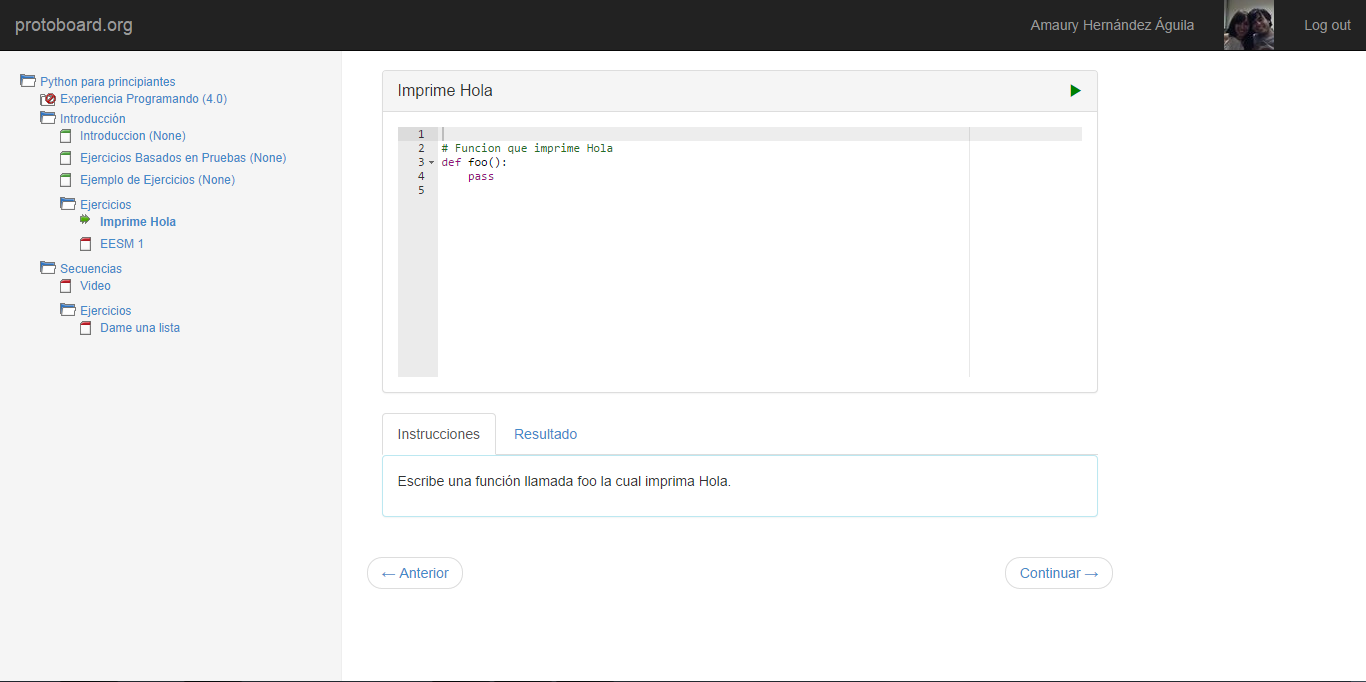
\includegraphics[width=10cm]{protoboard.png}}
  \caption{Interface of the Web Tutorial}
  \label{protoboard}
\end{figure}

\FloatBarrier

\subsubsection{Capturing the Keystroke and Mouse Data}

While a student is trying to solve an exercise, a script coded in JavaScript is running in the background, which captures every keystroke, mouse movement and mouse button press. Each capture of these events records a timestamp in milliseconds (using the method getTime() of JavaScript's built-in object Date) that describes when the event occurred. If the event is a keystroke, the script captures what key was specifically pressed (a JavaScript key code), and what type of event occurred (it can be either a key-down or a key-up event). If it is an event related to a mouse button press, the key code of that button is recorded, as well as the type of event occurred (key-down or key-up). Finally, if the event was a mouse movement, the mouse coordinates inside of the web browser is recorded. The script monitors the mouse position every 100 milliseconds, and if the position has changed, it records the new position.

\subsubsection{Capturing the Affective States}

In order to determine what affective states a student was experiencing, an Experience Sampling Method (ESM) was used \cite{esm}. After the students successfully solve a programming exercise, they are presented with an ESM survey that asks what they were feeling during their solving of the exercise. A very brief description is given about what to do in this survey, followed by two statements the students need to answer according to how they were feeling. As an example, the statement ``I was feeling frustrated'' is presented, and a student needs to answer either ``Strongly agree,'' ``Agree,'' ``Neutral,'' ``Disagree,'' and ``Strongly Disagree.'' %The full ESM survey is presented in Figure \ref{esm-survey}.

%% \begin{figure}[htp]
%%   \centerline{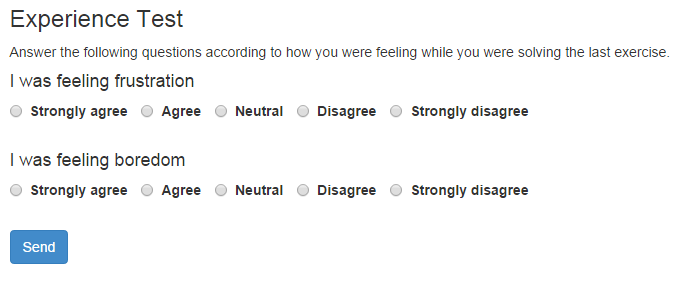
\includegraphics[width=10cm]{esm.png}}
%%   \label{esm-survey}
%%   \caption{Experience Sampling Method}
%% \end{figure}

%% \FloatBarrier

\subsubsection{Preprocessing of the Keystroke and Mouse Data}

The raw data obtained from the JavaScript script needs to be preprocessed in a way that results in a feature vector. Basically, this preprocessing consists in measuring the delays between key-down or key-up events of the keystrokes and mouse button presses a student performed during an exercise. The averages and standard deviations are calculated for each of these delays. To calculate these delays, the keystrokes are grouped in digraphs and trigraphs, as it is a common practice when dealing with Keystroke Dynamics \cite{digraph-trigraph}.

As most of the mouse button presses performed by a web site user are left button clicks, only these button presses are considered. To calculate the average and standard deviations of these presses, the delays between key-down and a key-up events of the left button clicks are used.

In addition to these averages and standard deviations of the delays between keystrokes and mouse button presses, the average and standard deviations of the number of total events contained in a digraph and a trigraph are calculated. These features are proposed and explained by Epp, Lippold, and Mandryk in \cite{keystroke-dynamics1}. Most of the times, a digraph should contain four events, while a trigraph should contain six events. However, sometimes an individual can start a digraph or a trigraph before ending the previous one. This additional features represent these particular cases, and could be meaningful for the estimation of an individual's affective states.

Regarding the mouse movements, the average and standard deviation of the duration of each mouse movement, and the averages and standard deviations of the movements in the X and Y axes, are calculated.

Lastly, a final feature is added to preprocessing of the data. The web tutorial recorded how many attempts a student required before successfully solving an exercise. This number of attempts is included in the final feature vector.

The final feature vector consists of 39 features.

%% \begin{center}
%%   \label{feature-vector}
%%   \begin{table}
%%     \caption{Tabla de características usadas}
%%   \tiny
%%   \begin{tabular}{| p{4cm} | p{8.2cm} |}
%%     \hline
%%     Nombre & Descripción \\ \hline
%%     2G\_1D2D\_MEAN & Tiempo promedio entre la 1ra (keydown) y 2da (keydown) tecla en un dígrafo\\ \hline
%%     2G\_1D2D\_SD & Desviación estándar de la característica anterior \\ \hline
%%     2G\_1Dur\_MEAN & Tiempo promedio entre el keydown y keyup de la 1ra
%%     tecla en un dígrafo \\ \hline
%%     2G\_1Dur\_SD & Desviación estándar de la característica anterior \\ \hline
%%     2G\_1KeyLat\_MEAN &  Tiempo promedio entre la 1ra (keyup) y el
%%     siguiente keydown en un dígrafo \\ \hline
%%     2G\_1KeyLat\_SD & Desviación estándar de la característica anterior \\ \hline
%%     2G\_2Dur\_MEAN & Tiempo promedio entre el keydown y keyup de la 2da
%%     tecla en un dígrafo \\ \hline
%%     2G\_2Dur\_SD & Desviación estándar de la característica anterior \\ \hline
%%     2G\_Dur\_MEAN & Tiempo promedio entre el primer keydown y el último
%%     keyup de un dígrafo \\ \hline
%%     2G\_Dur\_SD & Desviación estándar de la característica anterior \\ \hline
%%     2G\_NumEvents\_MEAN & Promedio del número de eventos contenidos en
%%     un dígrafo \\ \hline
%%     2G\_NumEvents\_SD & Desviación estándar de la característica anterior \\ \hline
%%     3G\_1D2D\_MEAN & Tiempo promedio entre la 1ra (keydown) y 2da
%%     (keydown) teclas de un trígrafo \\ \hline
%%     3G\_1D2D\_SD & Desviación estándar de la característica anterior \\ \hline
%%     3G\_1Dur\_MEAN & Tiempo promedio entre el keydown y keyup de la 1ra
%%     tecla en un trígrafo \\ \hline
%%     3G\_1Dur\_SD & Desviación estándar de la característica anterior \\ \hline
%%     3G\_1KeyLat\_MEAN & Tiempo promedio entre el keyup de la 1ra tecla y
%%     el siguiente keydown en un trígrafo\\ \hline
%%     3G\_1KeyLat\_SD & Desviación estándar de la característica anterior \\ \hline
%%     3G\_2D2D\_MEAN & Tiempo promedio entre la 2da (keydown) y 3ra
%%     (keydown) teclas en un trígrafo \\ \hline
%%     3G\_2D2D\_SD & Desviación estándar de la característica anterior \\ \hline
%%     3G\_2Dur\_MEAN & Tiempo promedio entre el keydown y keyup de la 2da
%%     tecla en un trígrafo \\ \hline
%%     3G\_2Dur\_SD & Desviación estándar de la característica anterior \\ \hline
%%     3G\_2KeyLat\_MEAN & Tiempo promedio entre el keyup de la 2da tecla y
%%     el siguiente keydown en un trígrafo\\ \hline
%%     3G\_2KeyLat\_SD & Desviación estándar de la característica anterior \\ \hline
%%     3G\_3Dur\_MEAN & Tiempo promedio entre el keydown y keyup de la
%%     última tecla en un trígrafo \\ \hline
%%     3G\_3Dur\_SD & Desviación estándar de la característica anterior \\ \hline
%%     3G\_Dur\_MEAN & Tiempo promedio entre el keydown de la 1ra tecla y
%%     el último keyup en un trígrafo \\ \hline
%%     3G\_Dur\_SD & Desviación estándar de la característica anterior \\ \hline
%%     3G\_NumEvents\_MEAN & Promedio del número de eventos contenidos en
%%     un trígrafo \\ \hline
%%     3G\_NumEvents\_SD & Desviación estándar de la característica anterior \\ \hline
%%     Mouse\_Presses\_Dur\_MEAN & Tiempo promedio entre el keydown y keyup
%%     de algún botón del ratón \\ \hline
%%     Mouse\_Presses\_Dur\_SD & Desviación estándar de la característica anterior \\ \hline
%%     Mouse\_Movement\_Dur\_MEAN & Tiempo promedio de todos los movimientos
%%     del ratón\\ \hline
%%     Mouse\_Movement\_Dur\_SD & Desviación estándar de la característica anterior \\ \hline
%%     Mouse\_Movement\_X\_MEAN & Promedio de la distancia recorrida en
%%     pixeles en la coordenada X por el ratón \\ \hline
%%     Mouse\_Movement\_X\_SD & Desviación estándar de la característica anterior \\ \hline
%%     Mouse\_Movement\_Y\_MEAN & Promedio de la distancia recorrida en
%%     pixeles en la coordenada Y por el ratón \\ \hline
%%     Mouse\_Movement\_Y\_SD & Desviación estándar de la característica anterior \\ \hline
%%     Attempts & Número de intentos requeridos para llegar a la
%%     solución del ejercicio \\ \hline
%%   \end{tabular}
%%   \end{table}
%% \end{center}

\subsubsection{Preprocessing of the Affective States}

The answers ``Strongly agree,'' and ``Agree'' were grouped into a single ``Agree'' class. The same was performed for the answers ``Strongly disagree,'' and ``Disagree.'' As a result, the feature vectors are now classified as either ``Agree,'' ``Neutral,'' or ``Disagree'', for each of the two affective states. The reason behind this decision is that the classifiers were performing poorly for such a big set of possible classes.

\subsubsection{Classification}

The feature vectors need to undergo an optimization process. This process consists on using a Genetic Algorithm to determine a subset of features that facilitates a classifier to obtain good results (this is explained in more detail in Section \ref{experiment}). The resulting feature vector is used as input to a classifier based on the k-Nearest Neighbors (k-NN) algorithm. In the end, two classifiers are trained: one for the frustration affective state, and another one for boredom.

\section{Experiment}
\label{experiment}

55 students with basic knowledge in software programming were asked to take the course presented in the web tutorial. The students were either studying Computer Systems Engineering, and were at least in their second year of study, or were students of a Master in Computer Science. Their ages were in the range of 18 to 30 years old. Although no experience in software programming was needed, as the web tutorial's course is of a very basic level, all the participants were required to had completed at least one course in software programming.

The goal for the students was to solve as many exercises in the web tutorial as they could. There was no time limit nor a minimum amount of time required for a participant while trying to solve the courses or complete the tutorial. The participants were able to stop and resume their interaction with the system at any time.

The participants' interaction generated a total of 142 feature vectors, meaning that each student solved an average of 2.58 exercises. The 39 features were associated with the answers of the ESM surveys the students had to answer after each exercise. As a result, the 142 feature vectors were used to train a classifier for each affective state. Each of these classifiers have the task of estimating if a given feature vector corresponds to either an ``Agree,'' ``Neutral,'' or ``Disagree'' class, for the frustration and boredom affective states.

At a first attempt at training the classifiers, bad results were being obtained. Accuracies of 50\% and below were frequent with each of the attempts, as well as Kappa Coefficients below 0.1.

The solution to this problem was to perform a selection of a subset of features in the feature vector. The hypothesis was that the classifiers were performing badly because of the high number of features, and because of the possible irrelevant features, i.e., features that don't help the classifier to improve its results. This preprocessing of the feature vector was done with RapidMiner's Optimize Selection operator based in Genetic Algorithms. Even with a population size of 700, the training and validation process had to be run several times before determining a satisfactory subset of features for both classifiers. In the end, the subset for the frustration classifier consists of 11 features, and the subset for the boredom classifier consists of 13 features.

For the validation of the results, 10-Fold Cross Validation was used.

\section{Results}
\label{results}

The results obtained with this method are very satisfactory, considering free-text KD was used. The accuracies and Kappa Coefficients obtained are close to what is usually obtained in fixed-text KD methods (for example, the results presented in \cite{keystroke-dynamics1}), and far superior to other research works involving free-text KD to predict affective states (for example, the results presented in \cite{keystroke-dynamics2}).

As can be seen in Figure \ref{accuracies-kappas}, both accuracies are well above 70\% which is considered a very good value in works pertaining to Affective Computing. In the case of the Kappa Coefficients (Figure \ref{accuracies-kappas}), it is usual to see values below 0.2 in methods involving free-text KD. In this case, both Kappas were close to 0.5. Specifically, the average and the standard deviation of the accuracies for the boredom and frustration classifiers were 83.81\%+/-5.51\%, and 74.00\%+/-6.07\%, respectively; and for the average and the standard deviation of the Kappas, they were 0.581+/-0.168 and 0.5+/-0.111, respectively. This means that, although both classifiers performed very well, the proposed method is more suitable for the classification of boredom.

\begin{figure}[htp]
  \centerline{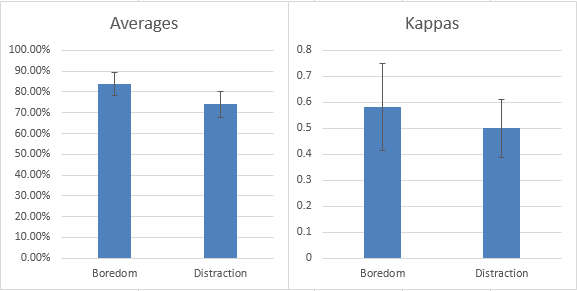
\includegraphics[width=10cm]{accuracy-kappa.png}}
  \caption{Accuracies and Kappa Coefficients for the Boredom and Frustration Classifiers}
  \label{accuracies-kappas}
\end{figure}

\section{Conclusion}
\label{conclusion}

The proposed method in this work obtained very satisfactory results. It is usual for a classification method based on free-text KD to obtain accuracies and Kappas below to their counterparts of fixed-text KD, and in this work the results obtained were similar to those works based on fixe-text KD. A possible explanation of this would be the addition of the MD features, and the additional preprocessing performed on the feature vectors.

As mentioned before, in the beginning of the Experiment, the proposed method was obtaining bad results, somewhat comparable to those usually obtained in methods based on free-text KD. However, after the optimization process (determining a subset of features), the results improved.

\section*{Acknowledgements}
\label{acknowledgements}

Lorem ipsum dolor sit amet, consectetur adipiscing elit. Nam pellentesque sodales odio a ultrices. Cras ac porta nulla. Sed varius ac leo ac luctus. Maecenas quis nisi eget lectus cursus venenatis eget ac nunc. Phasellus sed neque nec diam interdum suscipit. Proin vel lacinia magna. Suspendisse nec purus est. Nullam lacinia augue ultrices, fermentum eros quis, iaculis nisi. Sed eget est sit amet ipsum gravida facilisis. Praesent fermentum eros eget dolor mattis, sit amet rutrum purus faucibus. Pellentesque accumsan augue risus, nec malesuada ipsum lacinia in.

\begin{thebibliography}{4}
  
\bibitem{affective-computing} Picard, R.W.: Affective computing. MIT press (2000)
  
\bibitem{facial-expressions} El Kaliouby, R., and Robinson, P.: Real-time inference of complex mental states from facial expressions and head gestures. Real-time vision for human-computer interaction. Springer US, 181--200 (2005)

\bibitem{affective-simulation} Becker-Asano, C., and Wachsmuth, I.: Affect simulation with primary and secondary emotions. Intelligent Virtual Agents. Springer Berlin Heidelberg (2008)

\bibitem{autotutor} D'Mello, S., et al.: AutoTutor detects and responds to learners affective and cognitive states. Workshop on Emotional and Cognitive Issues at the International Conference on Intelligent Tutoring Systems (2008)

\bibitem{zoning-out} Drummond, J., and Litman, D.: In the zone: Towards detecting student zoning out using supervised machine learning. Intelligent Tutoring Systems. Springer Berlin Heidelberg (2010)

\bibitem{intrusive1} Jing, Z., and Barreto, A.: Stress detection in computer users based on digital signal processing of noninvasive physiological variables. Engineering in Medicine and Biology Society, 2006. EMBS'06. 28th Annual International Conference of the IEEE. IEEE (2006)

\bibitem{intrusive2} D'Mello, S., et al.: Integrating affect sensors in an intelligent tutoring system. Affective Interactions: The Computer in the Affective Loop Workshop (2005)

\bibitem{intrusive3} Arroyo, I., et al.: Emotion Sensors Go To School. AIED. Vol. 200 (2009)

\bibitem{free-text-fixed-text} Gunetti, D., and Picardi, C.: Keystroke analysis of free text. ACM Transactions on Information and System Security (TISSEC) 8.3, 312--347 (2005)

\bibitem{fixed-is-better} Janakiraman, R., and Sim, T.: Keystroke dynamics in a general setting. Advances in Biometrics. Springer Berlin Heidelberg, 584--593 (2007)

\bibitem{emotions-novices-programming} Bosch, N., D'Mello, S., and Mills, C.: What Emotions Do Novices Experience during Their First Computer Programming Learning Session. Artificial Intelligence in Education. Springer Berlin Heidelberg (2013)

\bibitem{emotions-novices-programming2} Rodrigo, M.M.T., et al.: Affective and behavioral predictors of novice programmer achievement. ACM SIGCSE Bulletin 41.3 156--160 (2009)

\bibitem{keystroke-dynamics1} Epp, C., Lippold, M., and Mandryk, R.L.: Identifying emotional states using keystroke dynamics. Proceedings of the SIGCHI Conference on Human Factors in Computing Systems. ACM (2011)

\bibitem{keystroke-dynamics2} Bixler, R., and D'Mello, S.: Detecting boredom and engagement during writing with keystroke analysis, task appraisals, and stable traits. Proceedings of the 2013 International Conference on Intelligent User Interfaces. ACM (2013)

\bibitem{mouse-dynamics1} Salmeron-Majadas, S., Santos, O.C., and Boticario, J.G.: Exploring indicators from keyboard and mouse interactions to predict the user affective state. Proceedings of the 7th International Conference on Educational Data Mining (EDM'14) (2014)

\bibitem{mouse-dynamics2} Bakhtiyari, K., and Husain, H.: Fuzzy Model in Human Emotions Recognition. 12th WSEAS International Conference on Applications of Computer Engineering (ACE '13) 77--82 (2014)

\bibitem{keystroke-mouse-review} Kolakowska, A.: A review of emotion recognition methods based on keystroke dynamics and mouse movements. 6th International Conference on on Human System Interaction (HSI). IEEE (2013)
  
%\bibitem{affect-aware-general1} Woolf, B., et al.: Affect-aware tutors: recognising and responding to student affect. International Journal of Learning Technology 4.3 129--164 (2009)
  
%\bibitem{affect-aware-general2} San Pedro, M.O.Z., et al.: Towards an understanding of affect and knowledge from student interaction with an Intelligent Tutoring System. Artificial Intelligence in Education. Springer Berlin Heidelberg (2013)

%\bibitem{affect-aware-general3} Wang, C.Y., et al.: Design an empathic virtual human to encourage and persuade learners in e-learning systems. Proceedings of the first ACM International Workshop on Multimedia Technologies for Distance Learning. ACM (2009)

\bibitem{esm} Larson, R., and Csikszentmihalyi, M.: The experience sampling method. New Directions for Methodology of Social & Behavioral Science (1983)

\bibitem{digraph-trigraph} Sim, T., and Janakiraman, R.: Are digraphs good for free-text keystroke dynamics. IEEE Conference on Computer Vision and Pattern Recognition, 2007 (CVPR'07). IEEE (2007)
  
\end{thebibliography}

\end{document}
